\documentclass[a4paper, 11pt]{article}

\usepackage{comment} % enables the use of multi-line comments (\ifx \fi)
\usepackage{lipsum} %This package just generates Lorem Ipsum filler text.
\usepackage{fullpage} % changes the margin
\usepackage{hyperref}

% \usepackage[backend=bibtex,style=verbose-trad2]{biblatex}
%\usepackage[backend=bibtex,
%  bibencoding=utf8
%  ]{biblatex}
% \usepackage[style=numeric-comp,natbib=true,backend=bibtex,bibencoding=utf8]{biblatex}
% \AtEveryBibitem{%
%   \clearfield{issn} % Remove issn
%   \clearfield{doi} % Remove doi
%   \clearfield{eprint} % Remove eprint
%   \clearfield{pages} % Remove pages number
%
%   \ifentrytype{online}{}{% Remove url except for @online
%     \clearfield{url}
%   }
% }
%\addbibresource{bib/mybib}
\usepackage{subfigure}
\usepackage{wrapfig}
\usepackage{xfrac}
\usepackage{multirow}
\usepackage{empheq}
\usepackage{mathtools}
\usepackage[sc]{mathpazo}

\usepackage[dvipsnames, table]{xcolor}

\usepackage{tabu}
\usepackage{longtable}

\usepackage{graphicx}
\usepackage{caption}
\captionsetup{%
  % font=footnotesize,% set font size to footnotesize
  labelfont=bf % bold label (e.g., Figure 3.2) font
}
\usepackage{array,booktabs}
\usepackage{framed}

\usepackage{amsmath}

\usepackage{pgfplots}        % make nice plots using raw data
\usepgfplotslibrary{external}
\usepackage{pstricks,pst-plot,psfrag}% Post-script graphics
\usetikzlibrary{plotmarks}
\usepackage{textcomp}
\usetikzlibrary{shapes,arrows}
 %define plots
\pgfplotsset{
  /pgfplots/xlabel near ticks/.style={
    /pgfplots/every axis x label/.style={
      at={(ticklabel cs:0.5)},anchor=near ticklabel
    }
  },
  /pgfplots/ylabel near ticks/.style={
    /pgfplots/every axis y label/.style={
      at={(ticklabel cs:0.5)},rotate=90,anchor=near ticklabel
    }
  }
}
\pgfplotsset{compat=newest}
\pgfplotsset{plot coordinates/math parser=false}

\usepackage{pgfgantt}

\setcounter{secnumdepth}{3} % only chapter and sections will be numbered
\setcounter{tocdepth}{1}    % entries down to \subsubsections in the TOC

\usepackage{enumitem}
%\usepackage{fouriernc}
% \usepackage{indentfirst}  % Causes the document to indent the first paragraph after a section
\usepackage{tabularx}


%%%%%%%%%%%%%%%%%%%% Color definitions %%%%%%%%%%%%%%%%%%%%%

\definecolor{aaublue}{RGB}{33,26,82}

\definecolor{tableHeader}{RGB}{211, 47, 47}
\definecolor{tableLineOne}{RGB}{245, 245, 245}
\definecolor{tableLineTwo}{RGB}{224, 224, 224}

\definecolor{bulletColor}{HTML}{323642}


%%%%%%%%%%%%%%%%%%%% New Commands %%%%%%%%%%%%%%%%%%%%%%%%%%%
\newcommand{\tableHeaderStyle}{
    \rowfont{\leavevmode\color{white}\bfseries}
    \rowcolor{tableHeader}
}
\newcommand{\degree}{$^\circ$}

% Black square bullets within lists
\newcommand{\localtextbulletone}{\textcolor{bulletColor}{\raisebox{.2ex}{\rule{1.0ex}{1.0ex}}}}
\renewcommand{\labelitemi}{\localtextbulletone}

% Table style definition
\taburowcolors[2] 2{tableLineOne .. tableLineTwo}
\tabulinesep = ^2mm_1mm
\everyrow{\tabucline[.4mm  white]{}}


\begin{document}
  \graphicspath{{./Figures/}}
%Header-Make sure you update this information!!!!
%\noindent
%\large\textbf{Post/Pre-Lab X Report} \hfill \textbf{FirstName LastName} \\
%\normalsize ECE 100-003 \hfill Teammates: Student1, Student2 \\
%Prof. Oruklu \hfill Lab Date: XX/XX/XX \\
%TA: Adam Sumner \hfill Due Date: XX/XX/XX
\pagenumbering{roman}
\tableofcontents
\newpage
\pagenumbering{arabic}
\section{Name of Candidate and Provisional Thesis Title}\label{sec:name_title}
\noindent
\begin{tabularx}{\textwidth}{l X}
\textbf{Candidate Name:} &\texttt{Sean \textsc{Thomas} }\\
\textbf{Provisional Thesis Title:} &\texttt{Smart Grippers: Conception of a novel type of actuator powered by Shape Memory Alloys}
\end{tabularx}

% \section{Keywords}\label{sec:keywords}
% \vspace{2pt}

\noindent ~~\textbf{Keywords \textendash}
Shape Memory Alloy, Buckled Beam, NiTiNOL, Shape Memory Effect, Bistable system, Self-switching, Modelling and Optimization, Printed Electronics

\section{Research Field and Motivation}\label{sec:research_mot}
\subsection{Motivation}\label{subsec:motivation}
In an era where manual assembly is no longer possible in the majority of developed countries, it is necessary for companies offering alternative solutions to stand out from their competitors. Manufacturers of assembly lines must modify the capabilities of their robots in order to be more competitive than the relocation of the assembly to countries with cheaper labour. In order to stand out, companies such as Mikron SA, seek to innovate grippers. The goal of this project would be to conceive and develop a novel and innovative type of Smart gripper. This small part plays a primordial role in the dynamics of the robot. Being at the end of the arm, a small gain in weight of this part would have great consequences on the acceleration and the maximum speed that the robot will be able to reach.

The \emph{Laboratory of Integrated Actuators}, along with a Swiss company, \emph{Mikron SA}, intend to develop a novel type of gripper that will harness the high work output per volume of smart materials. One such promising category of smart materials are the Shape Memory Alloys (SMA). This gripper would be designed to be lightweight and compact so as to be used as a pick and place gripper in clean room application. The project strives to investigate an innovative technology that will exploit the characteristics of this smart material to create an actuation system that is highly responsive, dynamic, lightweight and compact. These objective will motivate a doctoral thesis that is challenging and innovative.

\subsection{Research Field}\label{subsec:research_field}
Currently, few industrial actuators based on SMAs have been seen. This project first has to demonstrate the potential of such actuators as a gripper. Then optimisation of the right topology should reveal the full potential of SMA actuators in terms of time response and stroke. Heating the element is not the greatest challenge, the cooling time of the material must also be taken into account. It is important to note that it is often harder to dissipate heat rather than accumulate it. Thus, various heating and cooling solutions will be exploited and investigated during this project. Another challenge to overcome would be the limited fatigue life of such smart materials. The gripper should at the very least have a fatigue life in the order of $10^6$ cycles. The last challenge to over overcome would be to meet the requirements set by the currently used pneumatic grippers in industry.

This investigation will consider the thermal and mechanical aspect of the material so as to create a highly responsive and dynamic actuator capable of achieving the required force output and stroke of traditional grippers. The conception of the gripper will include optimization of the geometrical topology of the SMA blades and the use of bistable systems such as buckled beams to create dynamic and high stroke actuators. The command strategies of the actuator will also be an important area of study due to the fact that the actuation of the SMA will involve the precise control of its temperature and resistance.

The symbiosis of the bistable system and the SMA technology can result in an innovative gripper system. The interplay between these two domains will be studied and explored.

\subsection{Specifications of the gripper}\label{subsec:specifications}
The specifications of the actuator were obtained by comparing it with the specifications of the Schunk MPG-25 which is a common pneumatic gripper used in industry, more specifically the primary gripper used by Mikron SA.

\begin{table}[H]%{r}{5.5\textwidth}
  \centering
  \footnotesize
  \caption{Specifications of the required actuator}
  \label{tab:specs}
  \begin{tabu} to 0.5\textwidth {>{\bfseries}X[l, 3]  >{\bfseries}X[l, 1] X[r,1]}
      \tableHeaderStyle{tableRed}
      Criteria & Units & Value\\
      Stroke & mm & 3\\
      Grip force & N & 5\\
      Commutation time & ms & 50 - 100\\
      Weight & g & 100\\
      Precision/Repeatability & mm & 0.02\\
      Number of stable positions & \# & 2\\
      Volume & mm$^3$ & 120 \\
  \end{tabu}
\end{table}

Using the above specifications, the energy that the smart material must supply can be calculated to be approximately 15 mJ. This implies, for example, that for materials such as SMAs like NiTiNOL, the application would require only a volume of 1.5 mm$^3$.

\section{State of the Art} \label{sec:sota}
This section will discuss the existing smart materials that are currently studied and used in the domain of actuators. The different techniques and integration systems will also be presented with the goal to compare the various approaches currently used.

\subsection{Smart materials} \label{subsec:Smartmaterials}
In the field of engineering, ranging from haptics, automation and bio-medical fields, there has been a need  to create actuators that are lightweight, compact and having force output. This creates a need for materials that can deliver high forces and strokes while remaining light and small meaning that the materials need to have a high work output.

On the basis of creating an actuator that can meet the demands of the currently implemented strategies while at the same time pushing the limits of the current technology, a thorough investigation of the available smart materials must be conducted. These materials have the ability to react to an external stimulus such as thermal electrical or magnetic and are thus referred to as \emph{smart} or \emph{active materials}. These materials have an inherent property that allows them to be exploited with a specific external stimulus so as to alter their mechanical characteristics or to create self-sensing technology.

There exist numerous types of smart materials and based on their properties, they can be classified into many types such as \cite{damodharan_review_2018}:
\begin{itemize}
	\item Piezoelectric materials
	\item Magneto-strictive materials
	\item Electro-active polymers
	\item Shape Memory Alloys
\end{itemize}

The aim of this project is to adapt these aforementioned smart materials to harness their specific behaviour and fabricate smart actuators. This implies that the system that incorporates the material is equally critical for the conception of the actuator. This section of the report will delved into different strategies used to harness the specific behaviours of the smart materials and integrate them into actuators.

\subsubsection{Piezoelectric Materials}
Piezoelectric materials are a subgroup of smart materials that have the capability to produce voltages when a stress is applied. This behaviour is can also be expressed in the opposite direction i.e. a strain can be generated using an electric field. Piezoelectric materials are the most popular type of smart materials and the most commonly used piezoceramics, such as lead zirconate titanate, are available in the form of thin sheets. These sheets can then be stacked to create piezostack actuators.

\subsubsection{Magneto-strictive materials}
The magneto-strictive materials are category of smart materials that have the ability to alter their mechanical behaviour and shape when subjected to magnetic fields. Magnetic Shape Memory Alloys (MSMA) are a popular type of magnet0-strictive material. Here, the MSMA shows an interesting behaviour in which the material when deformed will tend to remain stable and retain its deformed shape. As the materials is introduced into a strong magnetic field, the crystals of the material are realigned and the material reverts back to its predeformed shape.

\subsubsection{Electro-Active polymers}

\subsubsection{Shape Memory Alloys}
Shape Memory Alloys (SMA) are a particular subgroup of smart materials that change their mechanical behaviour based on a thermal stimulus. Here, the material as with the MSMA, retains its shape when deformed and reverts back to its original shape when heated. Shape Memory Alloys (SMA) actuators provide us with an opportunity to create such actuators due to their high work output per volume which is around 10 $\mathrm{J}/\mathrm{cm}^3$\cite{MohdJani2014}. This can be a 10-fold increase when compared to pneumatic actuators. The SMA actuators are thus able to provide large amounts of force when compared to their volume, making them particularly useful in compact, lightweight actuators.

NiTiNOL, the most used SMA, contains an interesting property known as the Shape Memory Effect (SME), which allows the material to return to its unloaded state when it is heated above its transition temperature.

Shape memory alloys such NiTiNOL show two important properties: the Shape Memory Effect (SME) and Superelasticity (SE)\cite{Rao2015}. The property, this device aims to exploit is the SME. Materials exhibitng this property are able to return to a pre-defined shape when heated through a certain temperature range.

SMAs exist in various different stable phases which consists of the \emph{Martensitic (M)} phase and the \emph{Austenitic (A)} phase. The M phase can exist in either the \emph{Twinned M phase} or the \emph{Detwinned M phase} based on the stress experienced by the material. The SME is the effect that transforms the material from the A phase to its M phase, also known as the Martensitic transformation. The opposite transformation, from the M phase to the A phase, is known as Austenitic transformation. When the material reaches the Austentic transformation temperature ($\mathbf{A_s}$) threshold, the material will begin the Austenitic transformation. Inversely, as the material cools down to the Martensitic transformation temperature ($\mathbf{M_s}$), it will begin the Martensitic transformation. Since these transformations occur over a range in temperature, we must heat and cool well beyond the transformation temperatures.

The buckled SMA beam will make use of an SMA with a relatively high transformation temperature (with $A_s$ around 50\degreeC) and thus exists primarily in the M phase at room temperature. The phase transformations can be seen in figure \ref{fig:PhaseTransfDiagram}. When a mechanical load is applied to the SMA while in its M phase, the material shears on an atomic level and this allows it to deform through a detwinning process at relatively low stress levels. This process allows the material to deform up to strains of 8$\%$. Strains larger than this will cause dislocations which are irreversible. When the beam is then heated, the Austentite transformation from the detwinned M phase to the A phase, causes the beam to lose all the strain due to twinning, allowing the material to return to its original shape. This strain recovery allows the beam to revert to its pre-defined state while producing large forces.

\begin{figure}[H]
  \centering
  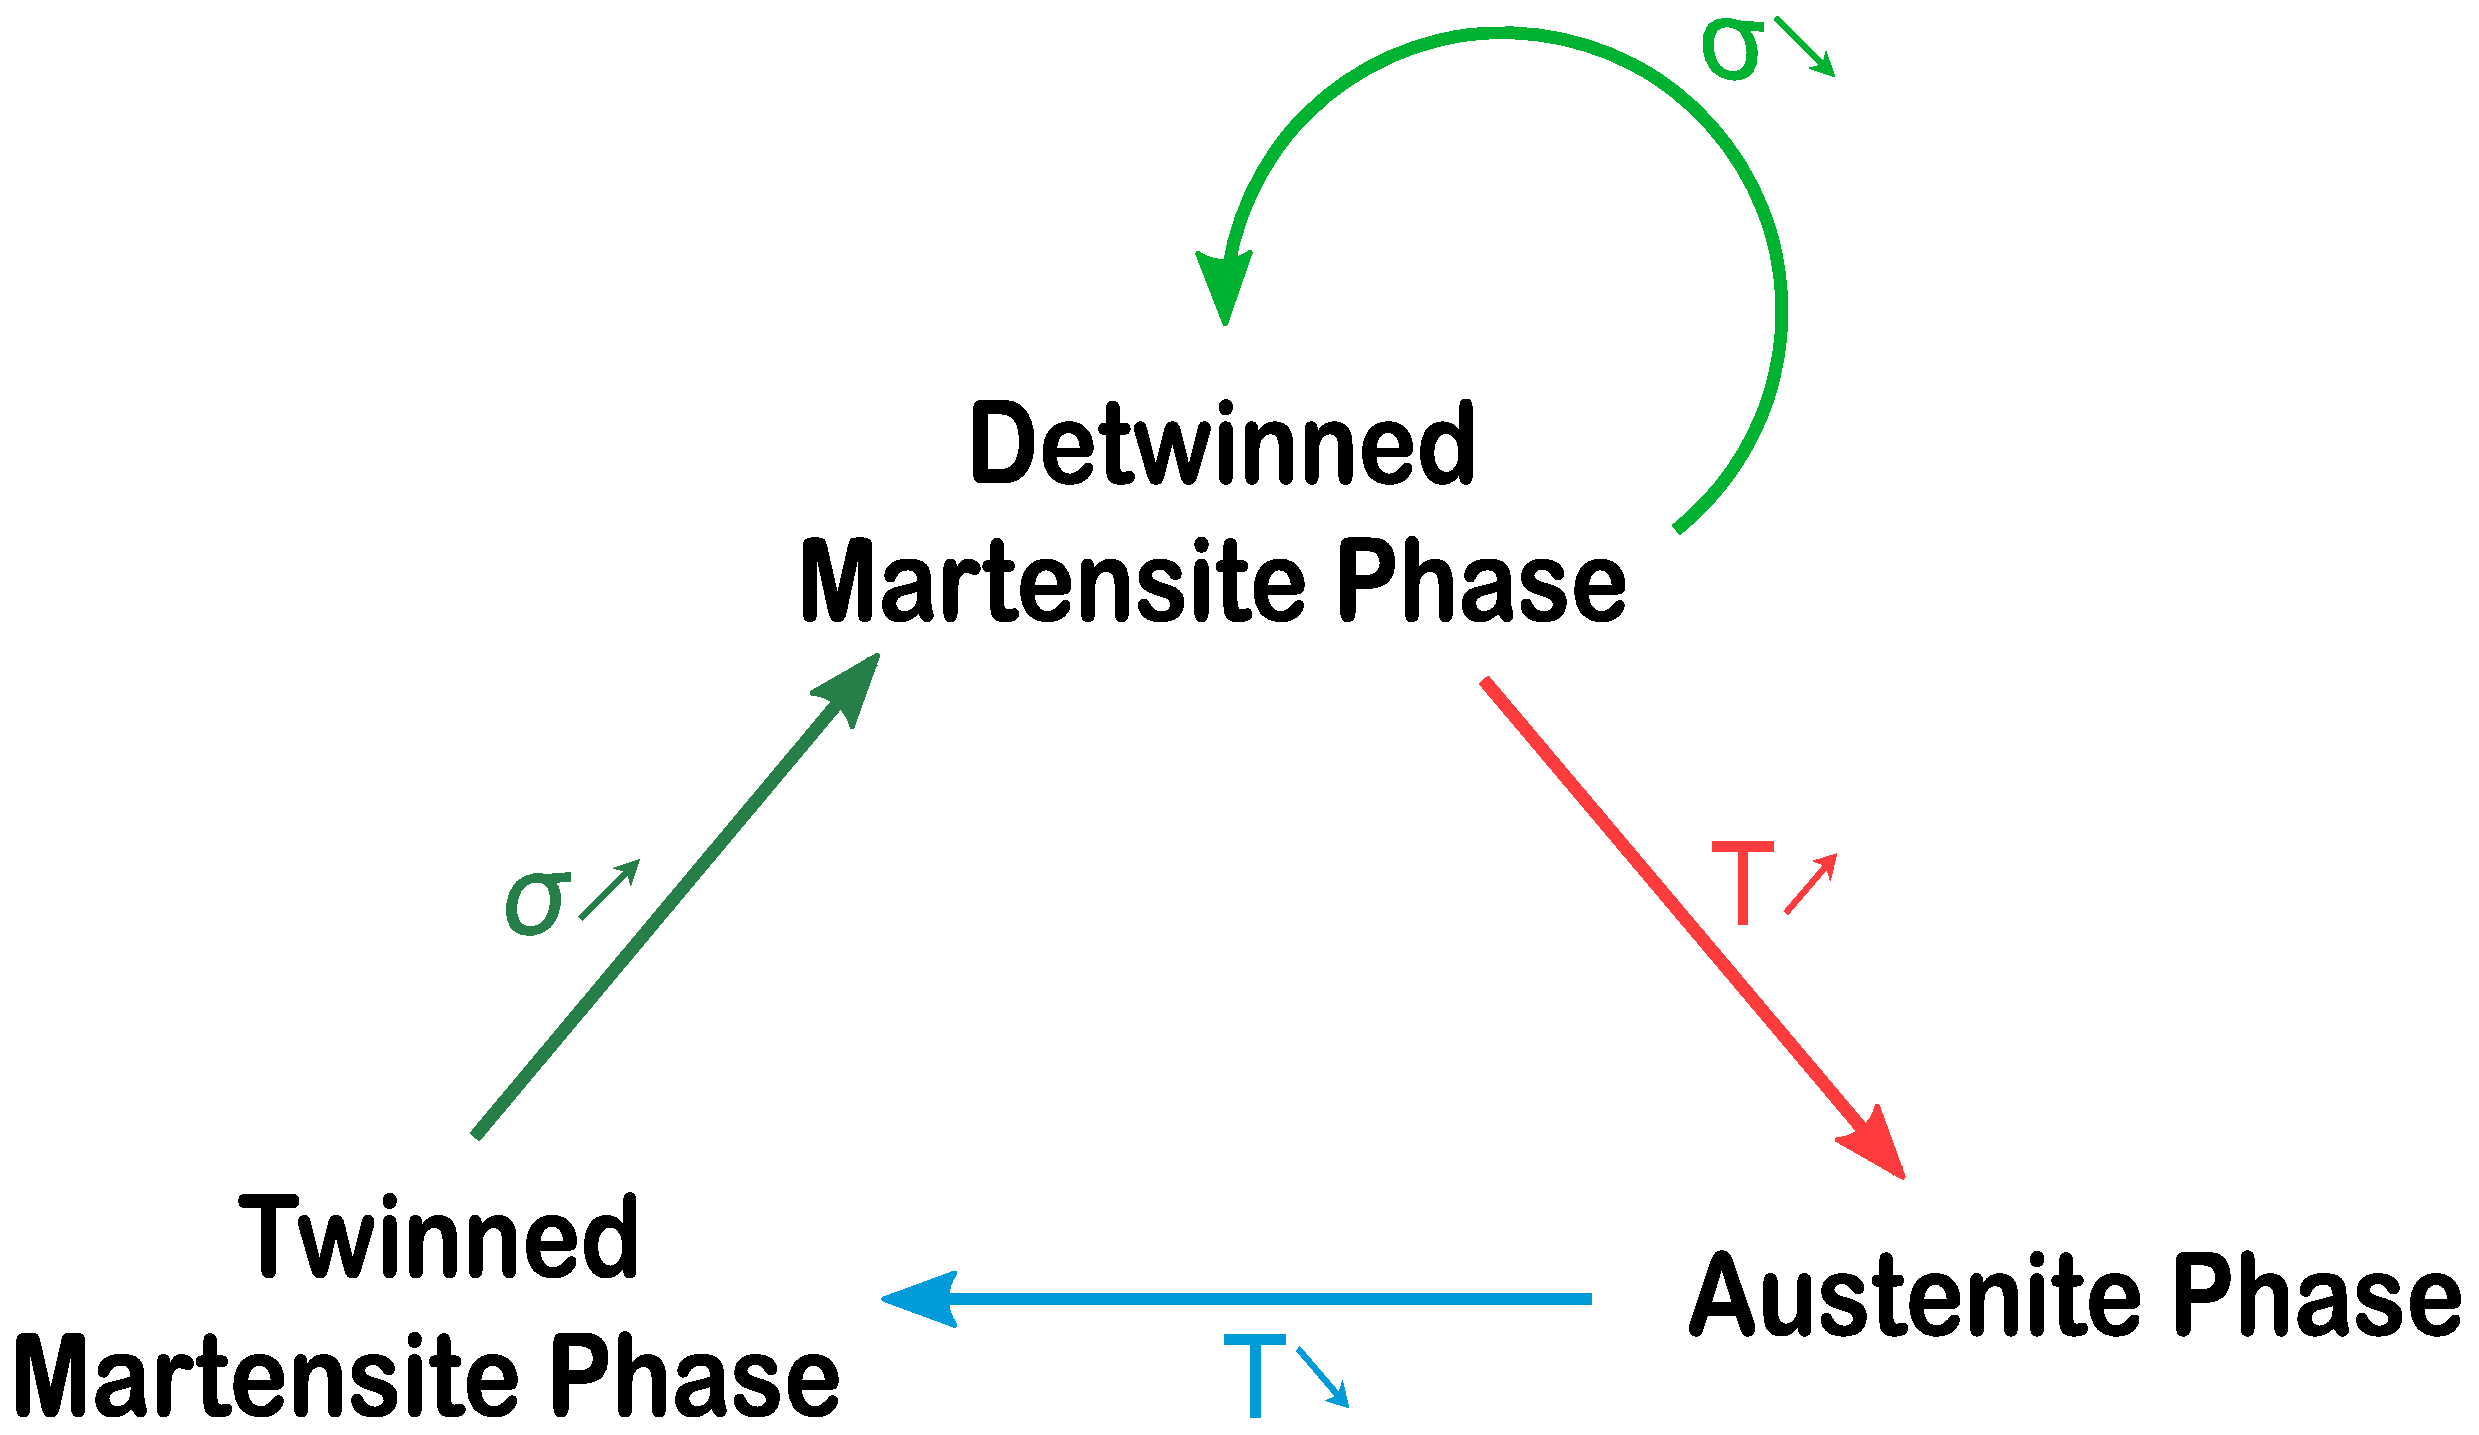
\includegraphics[width=0.5\textwidth]{Figures/Phase_Transf_Diagram_noText.eps}
  \caption{Phase transformation diagram of a shape memory alloy. Here $\sigma$ represents the stress created by mechanical loading and T represents the temperature change due to thermal loading.}
  \label{fig:PhaseTransfDiagram}
\end{figure}

\section{Work Accomplished}\label{sec:work_accomplished}

\section{Originality of the Research} \label{sec:originality}
The originality of this work lies in the pursuit of designing a gripper system that can harness the high work output of shape memory alloys. The gripper will be inspired by the various innovative smart technology explored within the state of the art. The state of the art shows that there exist many novel ideas for compact, light weight actuators using smart materials but non that are capable of delivering the high work output seen in SMAs. By harnessing the strengths of the SMA and the innovative strategies used in other smart material actuator systems, this research aims to explore the capabilities of the SMA material and develop an innovative gripper system. The following topics are expected to be studied over the course of this research project :
\begin{enumerate}
  \item Investigation of the SMA capabilities through the study of an analytical and finite element model
  \item Optimization of the topology of the active material component in the system for increased performances
  \item Optimization of heating and cooling strategies of the SMA so as to decrease response times and bandwidth
  \item Design and integration of a bistable system that incorporates an active smart material such as an SMA to achieve a responsive and powerful gripper system
\end{enumerate}

\section{Thesis Plan}
The following list presents a non-definitive thesis plan :
\begin{enumerate}
  \item Motivation of the Thesis
  \item State of the art : smart materials and actuation structures
  \item Topology optimisation
  \item Thermal optimisation
  \item Control
  \item Prototyping and validation
  \item Conclusion
\end{enumerate}

\section{Gantt Diagram}\label{sec:gantt}
\vspace{-1mm}
The follow diagram proposes a 4-year course for the doctorate. Some relevant conferences are displayed within the diagram.
%%PATO SUGGESTION
\begin{figure}[H]
\centering
\begin{ganttchart}
[
vgrid,
hgrid,
today=4,
newline shortcut=true,
bar label node/.append style={align=right},
x unit=.7 cm,
y unit chart=.4 cm,
today rule/.style={draw=tableRed, ultra thick},
milestone/.append style={fill=Goldenrod,rounded corners=.5pt,style={xscale=0.3}}%,
%milestone left shift=-.2,
]{1}{16}
\gantttitle{\footnotesize{2017}}{1}
\gantttitle{2018}{4}
\gantttitle{2019}{4}
\gantttitle{2020}{4}
\gantttitle{2021}{3} \\
%%%CTI
%\ganttbar[bar/.append style={fill=magenta}]{Modelling Bearingless}{1}{3}\\
%\ganttbar[bar/.append style={fill=magenta}]{Conception and Optimization}{3}{6}\\
%\ganttbar[bar/.append style={fill=magenta}]{Realization of Ventilation Prototype}{6}{8}\\
%\ganttbar[bar/.append style={fill=magenta}]{Command Electronics}{8}{10}
%%%
%\ganttnewline[thick, blue]
\ganttbar[
bar/.append style={fill=color1}
]{\footnotesize{Literature Review}}{1}{2}\\

\ganttbar[
bar/.append style={fill=color1}
]{\footnotesize{Modeling of SMAs}}{2}{3}

\ganttmilestone[
inline, milestone inline label node/.append style={right=1mm},
milestone/.append style={fill=greenColor3},
milestone left shift=.4,
milestone right shift=.4,
]{\href{http://www.icems2018.com/}{ICEMS 18'}}{4}\\

\ganttbar[
bar/.append style={fill=color2}
]{\footnotesize{Catalogue of Bistable Solutions}}{3}{3}

\ganttmilestone[
inline, milestone inline label node/.append style={right=1mm},
milestone/.append style={fill=greenColor3},
milestone left shift=.6,
milestone right shift=.6,
]{\href{http://www.icems2018.com/}{ICEMS 18'}}{4}\\

\ganttbar[bar/.append style={fill=color2}]{\footnotesize{FEM Analysis of Systems}}{3}{4}

\ganttmilestone[
inline, milestone inline label node/.append style={right=1mm},
milestone/.append style={fill=greenColor1},
milestone left shift=.0,
milestone right shift=.0,
]{\href{https://ldia2019.epfl.ch/}{LDIA 19'}}{6}\\

%\ganttmilestone[inline]{ICEMS}{5}\\
\ganttbar[
bar/.append style={fill=color3}
]{\footnotesize{Time Response Enhancement}}{3}{6}

\ganttmilestone[
inline, milestone inline label node/.append style={right=1mm},
milestone/.append style={fill=greenColor1},
milestone left shift=.0,
milestone right shift=.0,
]{\href{http://www.aim2019.org/}{AIM 19'}}{8}\\

\ganttbar[
bar/.append style={fill=color3}
]{\footnotesize{SMA Integration Analysis}}{6}{8}\\

\ganttbar[
bar/.append style={fill=color3}
]{\footnotesize{Electrode Deposition Analysis}}{8}{9}\\

\ganttbar[
bar/.append style={fill=color4}
]{\footnotesize{1$^{\text{st.}}$ Prototype}}{10}{12}\\

% \ganttmilestone[
% inline, milestone inline label node/.append style={right=1mm},
% milestone left shift=.0,
% milestone right shift=.0,
% ]{\href{https://ias.ieee.org/events-conferences/conference-schedule.html}{APEC 20'}}{12}\\

\ganttbar[
bar/.append style={fill=color4}
]{\footnotesize{Prototyping and Validation}}{12}{14}\\

\ganttbar[bar/.append style={fill=color5}]{\footnotesize{Redaction}}{15}{16}
\end{ganttchart}
\label{fig:gantt}
\vspace{-10mm}
\end{figure}

\section{Publications}
\begin{itemize}
  \item \emph{Accepted:} S. Thomas, M. Almanza, Y. Civet, and Y. Perriard, ``Actuation Displacement Analysis of a Self-Switching Shape Memory Alloy Buckled Beam'', in \emph{International Conference on Electrical Machines and Systems}, Jeju, 2018, p. 7.
  \item \emph{Accepted:} S. Thomas, P. Peralta, R. Mottet, M. Lehmann, Y. Civet, and Y. Perriard, ``Analysis and Reduction of Time Response in Thermally Activated Shape Memory Alloys'', in \emph{International Conference on Electrical Machines and Systems}, Jeju, 2018, p. 6.
\end{itemize}


%\printbibliography[heading=bibintoc]
%\label{bib:mybiblio}
%\section*{Problem Statement}
%Put your Problem statement here! Example of a Citation\cite[p.219]{Robotics}. Here's Another Citation\cite{Flueck}
%
%\section*{Investigation/Research}
%\lipsum[2]
%
%\section*{Alternative Solutions}
%\lipsum[3]
%
%\section*{Optimum Solution}
%\lipsum[4]
%% to comment sections out, use the command \ifx and \fi. Use this technique when writing your pre lab. For example, to comment something out I would do:
%%  \ifx
%%	\begin{itemize}
%%		\item item1
%%		\item item2
%%	\end{itemize}
%%  \fi
%
%\section*{Construction/Implementation}
%\lipsum[5]
%
%\section*{Analysis \& Testing}
%\lipsum[6]
%
%\section*{Final Evaluation}
%\lipsum[7]
%
%\section*{Attachments}
%%Make sure to change these
%Lab Notes, HelloWorld.ic, FooBar.ic
%%\fi %comment me out
%
%\begin{thebibliography}{9}
%\bibitem{Robotics} Fred G. Martin \emph{Robotics Explorations: A Hands-On Introduction to Engineering}. New Jersey: Prentice Hall.
%\bibitem{Flueck}  Flueck, Alexander J. 2005. \emph{ECE 100}[online]. Chicago: Illinois Institute of Technology, Electrical and Computer Engineering Department, 2005 [cited 30
%August 2005]. Available from World Wide Web: (http://www.ece.iit.edu/~flueck/ece100).
%\end{thebibliography}
\bibliographystyle{ieeetr}
\bibliography{Candidacy_ST_RevB}

\end{document}
